\documentclass[12pt, a4paper]{article}

% Gold-Standard Academic Typography & Encoding Packages
\usepackage[T1]{fontenc}
\usepackage{lmodern}
\usepackage[utf8]{inputenc}
\usepackage{microtype}
\usepackage[margin=1.0in]{geometry}
\setlength{\headheight}{20pt}

% Line & Paragraph Spacing Packages
\usepackage{setspace}
\onehalfspacing
\usepackage[skip=0.8em, indent=0pt]{parskip}

% Styling & Color Packages
\usepackage{xcolor}
\definecolor{navyblue}{RGB}{15, 42, 74}
\definecolor{slateblue}{RGB}{30, 58, 138}
\definecolor{darkgray}{RGB}{51, 65, 85}

% Section Heading Customization
\usepackage{titlesec}
\titleformat{\section}{\Large\bfseries\color{navyblue}}{\thesection}{1em}{}[\vspace{0.2em}\hrule height 0.6pt]
\titleformat{\subsection}{\large\bfseries\color{slateblue}}{\thesubsection}{0.8em}{}
\titlespacing*{\section}{0pt}{3.0ex plus 1ex minus .2ex}{2.0ex plus .2ex}
\titlespacing*{\subsection}{0pt}{2.5ex plus 1ex minus .2ex}{1.2ex plus .2ex}

% List & Table Formatting Packages
\usepackage{enumitem}
\setlist[itemize]{itemsep=0.4em, topsep=0.4em, parsep=0.2em, leftmargin=1.5em}
\setlist[enumerate]{itemsep=0.5em, topsep=0.5em, parsep=0.2em, leftmargin=1.5em}
\usepackage{booktabs}
\usepackage{float}
\usepackage{array}
\usepackage{tabularx}
\usepackage{caption}

% Additional Core Packages
\usepackage{graphicx}
\usepackage{hyperref}
\usepackage{amsmath, amssymb}
\usepackage{fancyhdr}

% Hyperref Setup
\hypersetup{
    colorlinks=true,
    linkcolor=navyblue,
    citecolor=navyblue,
    urlcolor=navyblue,
    pdftitle={Project Proposal 2.0 - CampusCare},
    pdfauthor={CampusCare Development Team}
}

% Header and Footer Setup
\pagestyle{fancy}
\fancyhf{}
\rhead{\small \textbf{\color{darkgray}Software Engineering Project Proposal 2.0}}
\lhead{\small \textbf{\color{darkgray}CampusCare Proposal}}
\rfoot{\small \color{darkgray}Page \thepage}
\lfoot{\small \color{darkgray}University Infrastructure \& Facility Management}
\renewcommand{\headrulewidth}{0.4pt}
\renewcommand{\footrulewidth}{0.4pt}

\begin{document}

% =========================================================
% COVER PAGE
% =========================================================
\begin{titlepage}
    \centering
    
    % University Logo
    
\includegraphics[width=0.25\textwidth]{../srs/uits_logo.png}\\[1.0cm]
    
    {\Large \textbf{University of Information Technology and Sciences (UITS)}}\\[0.3cm]
    {\large Department of Computer Science and Engineering}\\[1.2cm]
    
    {\Large \textbf{COURSE:}} Software Project Design and Development (CSE 416)\\[1.0cm]
    
    \rule{\linewidth}{0.6mm}\\[0.4cm]
    {\LARGE \textbf{\color{navyblue}PROJECT PROPOSAL 2.0}}\\[0.2cm]
    {\large \textbf{Project Title: CampusCare}}\\[0.1cm]
    {\small Centralized University Complaint Management System}\\[0.4cm]
    \rule{\linewidth}{0.6mm}\\[1.5cm]
    
\begin{minipage}{0.48\textwidth}
    \begin{flushleft} \large
        \textbf{Submitted To:}\\[0.2cm]
        \textbf{Dr. Mahfida Amjad Dipa}\\
        Assistant Professor\\
        Department of CSE, UITS
    \end{flushleft}
\end{minipage}
\hfill
\begin{minipage}{0.48\textwidth}
    \begin{flushright} \large
        \textbf{Submitted By (Group Members):}\\[0.2cm]
        \textbf{Rudro Antony Mrong}\\
        ID: 0432320005101059\\[0.2cm]
        \textbf{Md. Masud Rahman}\\
        ID: 0432320005101064\\[0.2cm]
        \textbf{Shafayat Hossain Shafin}\\
        ID: 0432320005101088
    \end{flushright}
\end{minipage}
    
    \vfill
    {\large Submission Date: August 2026}
\end{titlepage}

\newpage
\tableofcontents
\newpage

% =========================================================
% 1. OBJECTIVES
% =========================================================
\section{Objectives}

\subsection{Primary Objective}
To design, develop, and deploy a responsive campus facility management platform that centralizes complaint submission, automated Service Level Agreement (SLA) deadline tracking, role-based dispatching, rate-limited submission APIs, and audit logging within a unified system.

\subsection{Quantifiable and Operational Objectives}
\begin{enumerate}
    \item \textbf{Resolution Acceleration:} Reduce average complaint resolution lifecycle time across campus facility operations by 40\%.
    \item \textbf{Centralized Tracking:} Achieve 100\% centralized tracking of submitted service requests through an authenticated single submission pipeline.
    \item \textbf{SLA Compliance:} Maintain institutional SLA compliance above 85\% across all complaint priority levels (\texttt{Critical: 4h}, \texttt{High: 24h}, \texttt{Medium: 72h}, \texttt{Low: 168h}).
    \item \textbf{Database Query Performance:} Maintain database response latencies below 500ms for administrative reporting queries on datasets up to 10,000 records.
    \item \textbf{Audit Traceability:} Maintain 100\% audit coverage for ticket status transitions and staff assignment updates stored in an immutable audit ledger (\texttt{audit\_logs}).
\end{enumerate}

% =========================================================
% 2. SCOPE
% =========================================================
\section{Scope}

\subsection{In-Scope (Minimum Viable Product - MVP)}
The scope for the initial system release encompasses:

\begin{itemize}
    \item \textbf{Authentication and Security:} Email/password authentication via \texttt{@supabase/ssr}, \texttt{HttpOnly} session cookie management, Next.js Edge proxy middleware for role-based route protection (\texttt{Student}, \texttt{Staff}, \texttt{Admin}), and Upstash Redis sliding-window rate limiting (\texttt{@upstash/ratelimit}) on submission endpoints.
    \item \textbf{Student Module:} Dashboard with metric cards, complaint submission form with custom animated dropdown pickers and photo proof uploads, human-readable Complaint ID generation (\texttt{CMP-YYYY-XXXX}), real-time ticket timeline tracking, and resolution confirmation/rejection workflow.
    \item \textbf{Staff Module:} Departmental ticket queues, visual SLA deadline warning indicators, state transition controls (\texttt{Assigned} $\rightarrow$ \texttt{In Progress} $\rightarrow$ \texttt{Resolved}), internal progress note logs, manual SLA target date overrides with reason notes, and completion photo proof uploads.
    \item \textbf{Admin Module:} Global master ticket table with multi-parameter filtering using \texttt{@tanstack/react-table}, ticket reassignment and priority override controls, user role promotion and department assignment desk, category/department taxonomy management, and operational analytics charts.
    \item \textbf{Database and Storage Infrastructure:} PostgreSQL relational schema with Row Level Security (RLS) policies utilizing \texttt{SECURITY DEFINER} helper functions to prevent policy recursion, foreign key constraints, automated ticket sequence triggers, and an immutable audit log table (\texttt{audit\_logs}).
\end{itemize}

\subsection{Out-of-Scope (Future Iterations - Version 2.0)}
The following capabilities are excluded from the initial release and reserved for future project phases:
\begin{itemize}
    \item Automated AI complaint classification and duplicate ticket detection.
    \item Real-time WebSocket push notifications and external transactional email dispatching (e.g., Resend / SendGrid API).
    \item Native mobile applications for iOS/Android operational staff (React Native / Expo).
    \item Multi-campus organizational hierarchy support across geographically separated university branches.
\end{itemize}

\newpage

% =========================================================
% 3. FEASIBILITY STUDY
% =========================================================
\section{Feasibility Study}

\subsection{Technical Feasibility}
The system leverages Next.js 16 (App Router), React 19, TypeScript, Tailwind CSS, \texttt{@tanstack/react-table}, and Supabase (PostgreSQL). This stack provides standard SSR support, strong type safety, and clean separation of client and server logic. Supabase Row Level Security (RLS) combined with \texttt{SECURITY DEFINER} SQL helper functions enforces strict role-based data isolation at the database layer. Upstash Redis handles request rate limiting to protect public endpoints against abuse.

\subsection{Operational Feasibility}
The UI is built using the Caring Campus Green design system with responsive layouts supporting viewports down to 320px width and high-contrast text meeting WCAG standards. The system reflects standard university facility workflows (\texttt{Student reports} $\rightarrow$ \texttt{System/Admin assigns} $\rightarrow$ \texttt{Staff resolves} $\rightarrow$ \texttt{Student verifies}), requiring minimal training for campus maintenance personnel and students.

\subsection{Economic Feasibility}
Next.js, React, Tailwind CSS, and PostgreSQL incur zero software licensing fees. Hosting on Vercel and Supabase keeps operational overhead low, starting on free dev tiers and scaling to modest Pro tiers (\$45/month total) for production workloads, significantly reducing manual administrative labor costs.

\newpage

% =========================================================
% 4. WORK BREAKDOWN STRUCTURE (WBS)
% =========================================================
\section{Work Breakdown Structure (WBS)}

\begin{figure}[H]
    \centering
    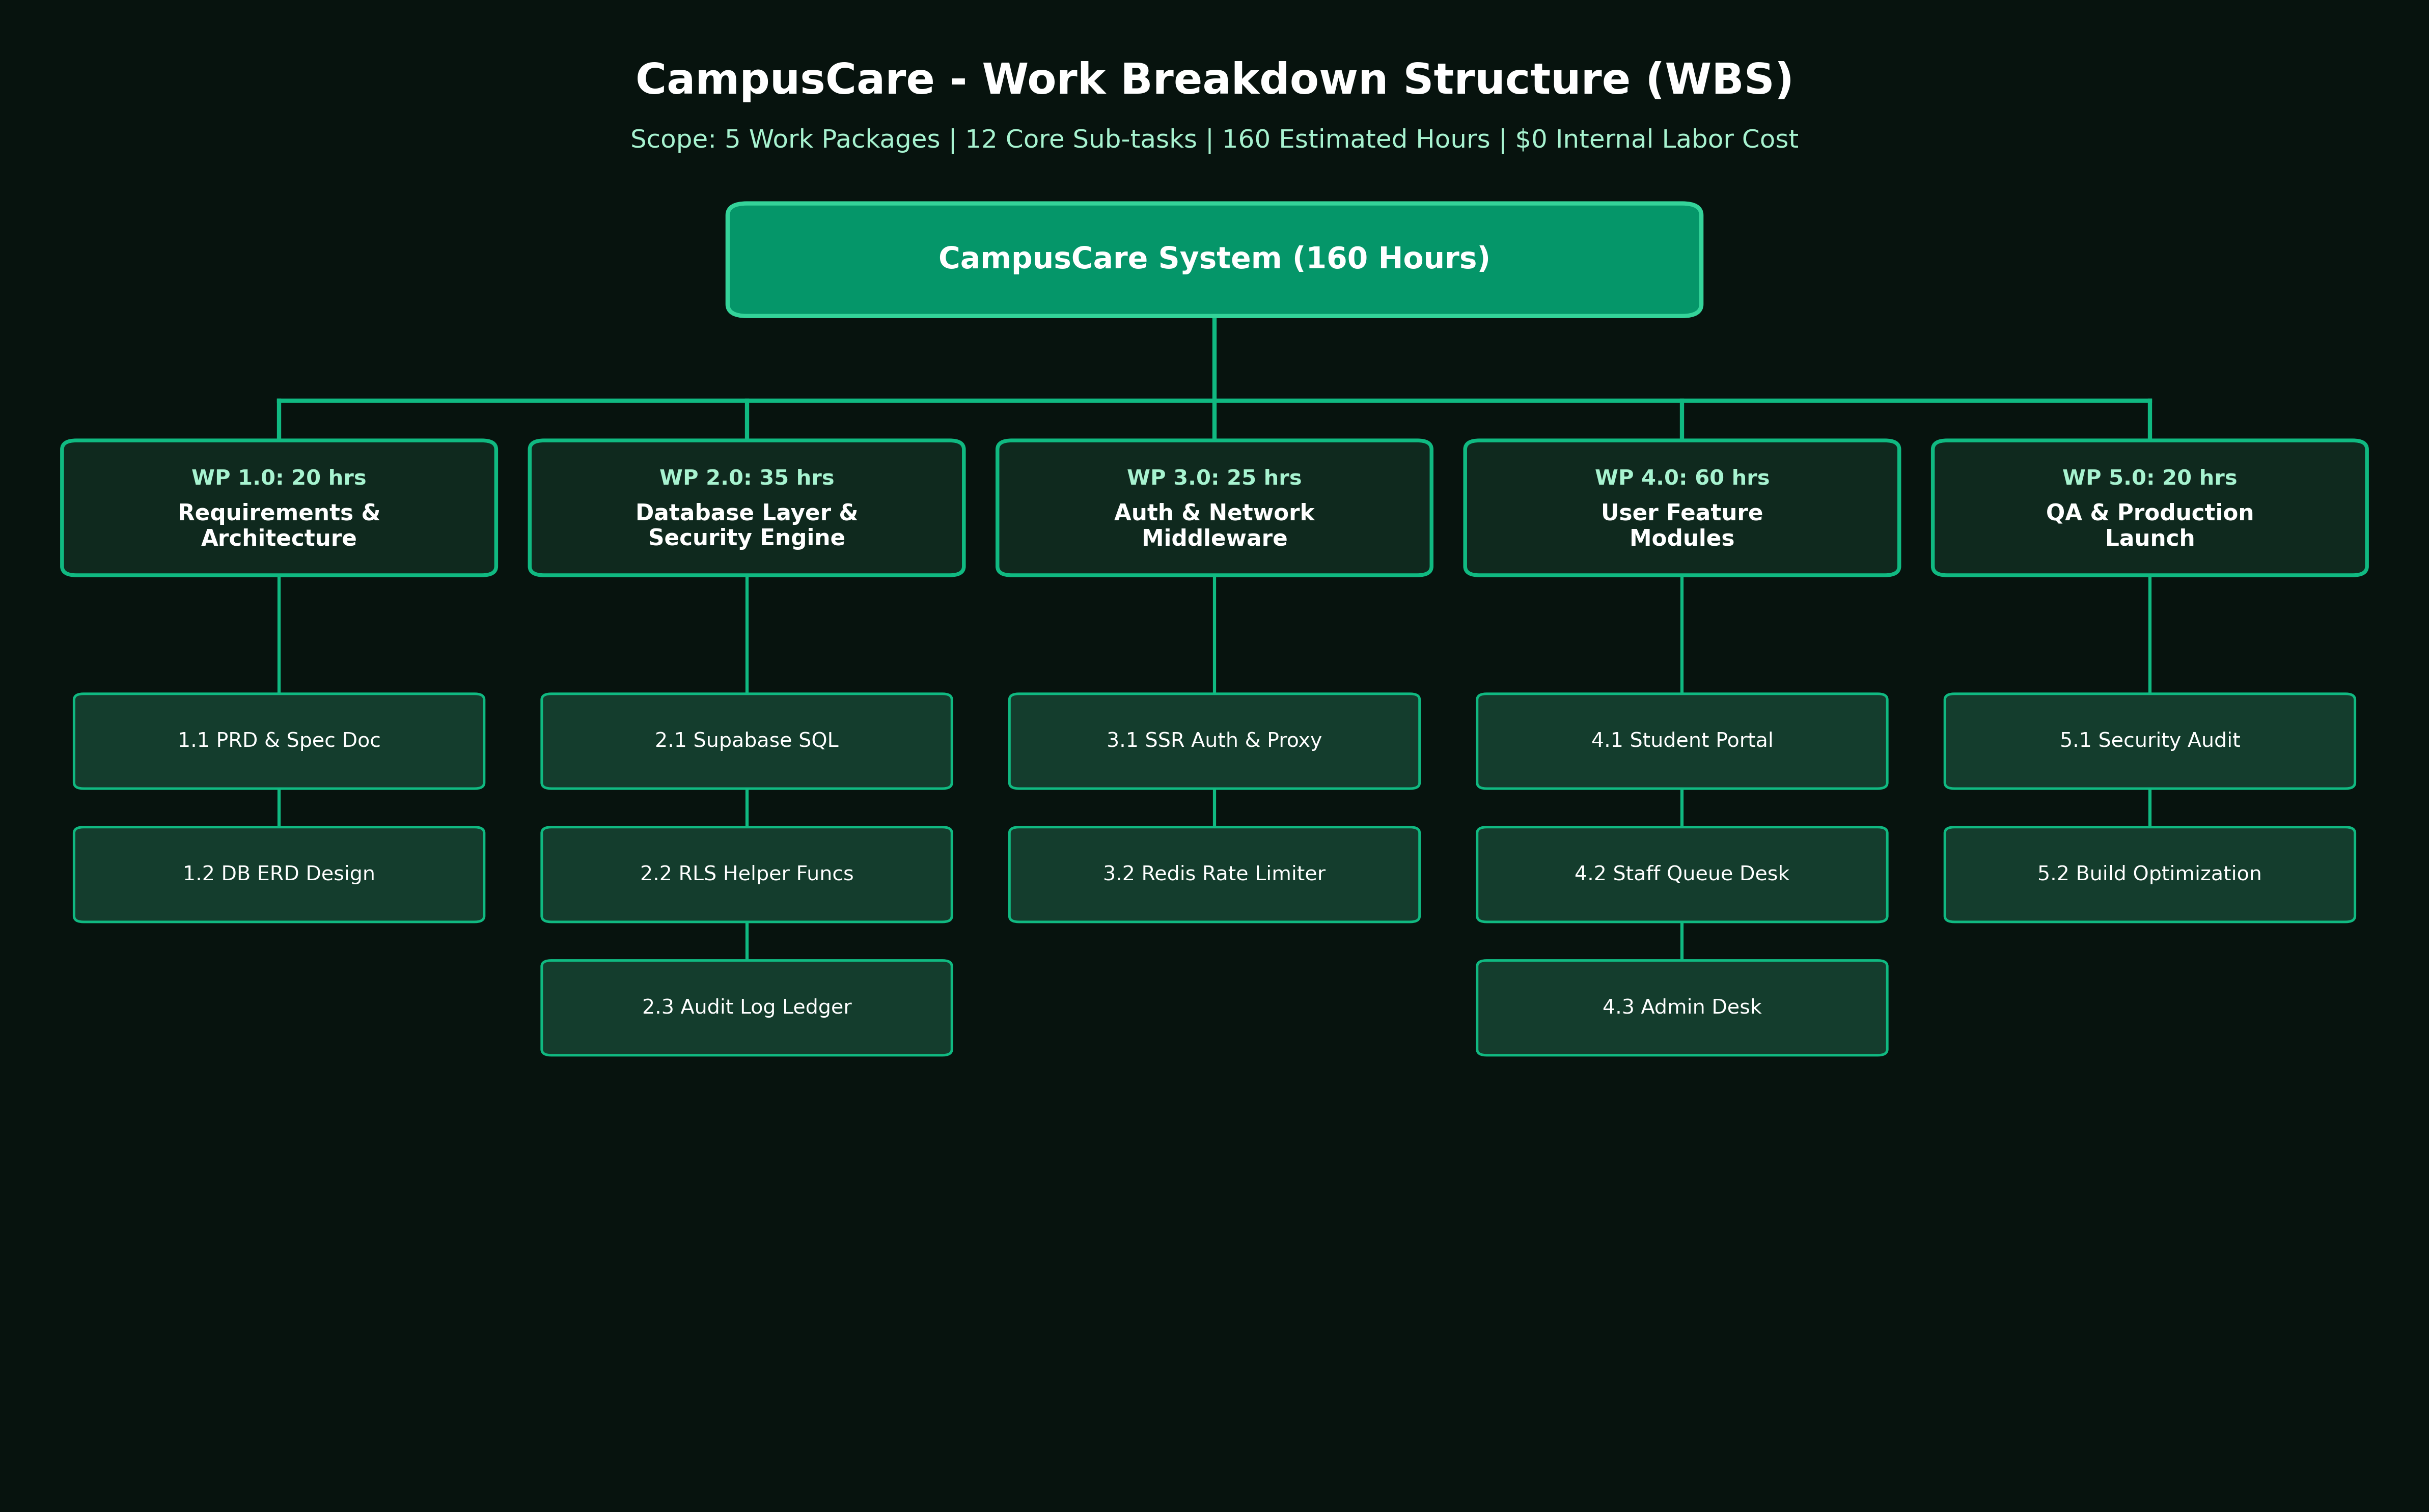
\includegraphics[width=0.95\textwidth]{../diagrams/campuscare_wbs.png}
    \caption{CampusCare Work Breakdown Structure (WBS) Tree Diagram.}
    \label{fig:wbs}
\end{figure}

\begin{table}[H]
\centering
\small
\begin{tabularx}{\textwidth}{l X c c}
\toprule
\textbf{Work Package} & \textbf{Title and Deliverables} & \textbf{Labor (Hours)} & \textbf{Cost (USD)} \\
\midrule
\textbf{WP 1.0} & Requirements and Architecture (PRD, Spec, ERD) & 20 hrs & \$0.00 \\
\textbf{WP 2.0} & Database and Security (PostgreSQL, RLS, Audit Log) & 35 hrs & \$0.00 \\
\textbf{WP 3.0} & Auth and Middleware (\texttt{@supabase/ssr}, Proxy, Redis) & 25 hrs & \$0.00 \\
\textbf{WP 4.0} & Core Modules (Student, Staff, Admin Desks) & 60 hrs & \$0.00 \\
\textbf{WP 5.0} & QA and Launch (Security Audit, WCAG, Build Optimization) & 20 hrs & \$0.00 \\
\midrule
\textbf{Total Project} & \textbf{5 Work Packages (12 Sub-tasks)} & \textbf{160 Hours} & \textbf{\$0.00} \\
\bottomrule
\end{tabularx}
\caption{Work Package Task and Labor Costing Breakdown.}
\end{table}

\newpage

% =========================================================
% 5. GANTT CHART
% =========================================================
\section{Gantt Chart and Project Timeline}

\begin{figure}[H]
    \centering
    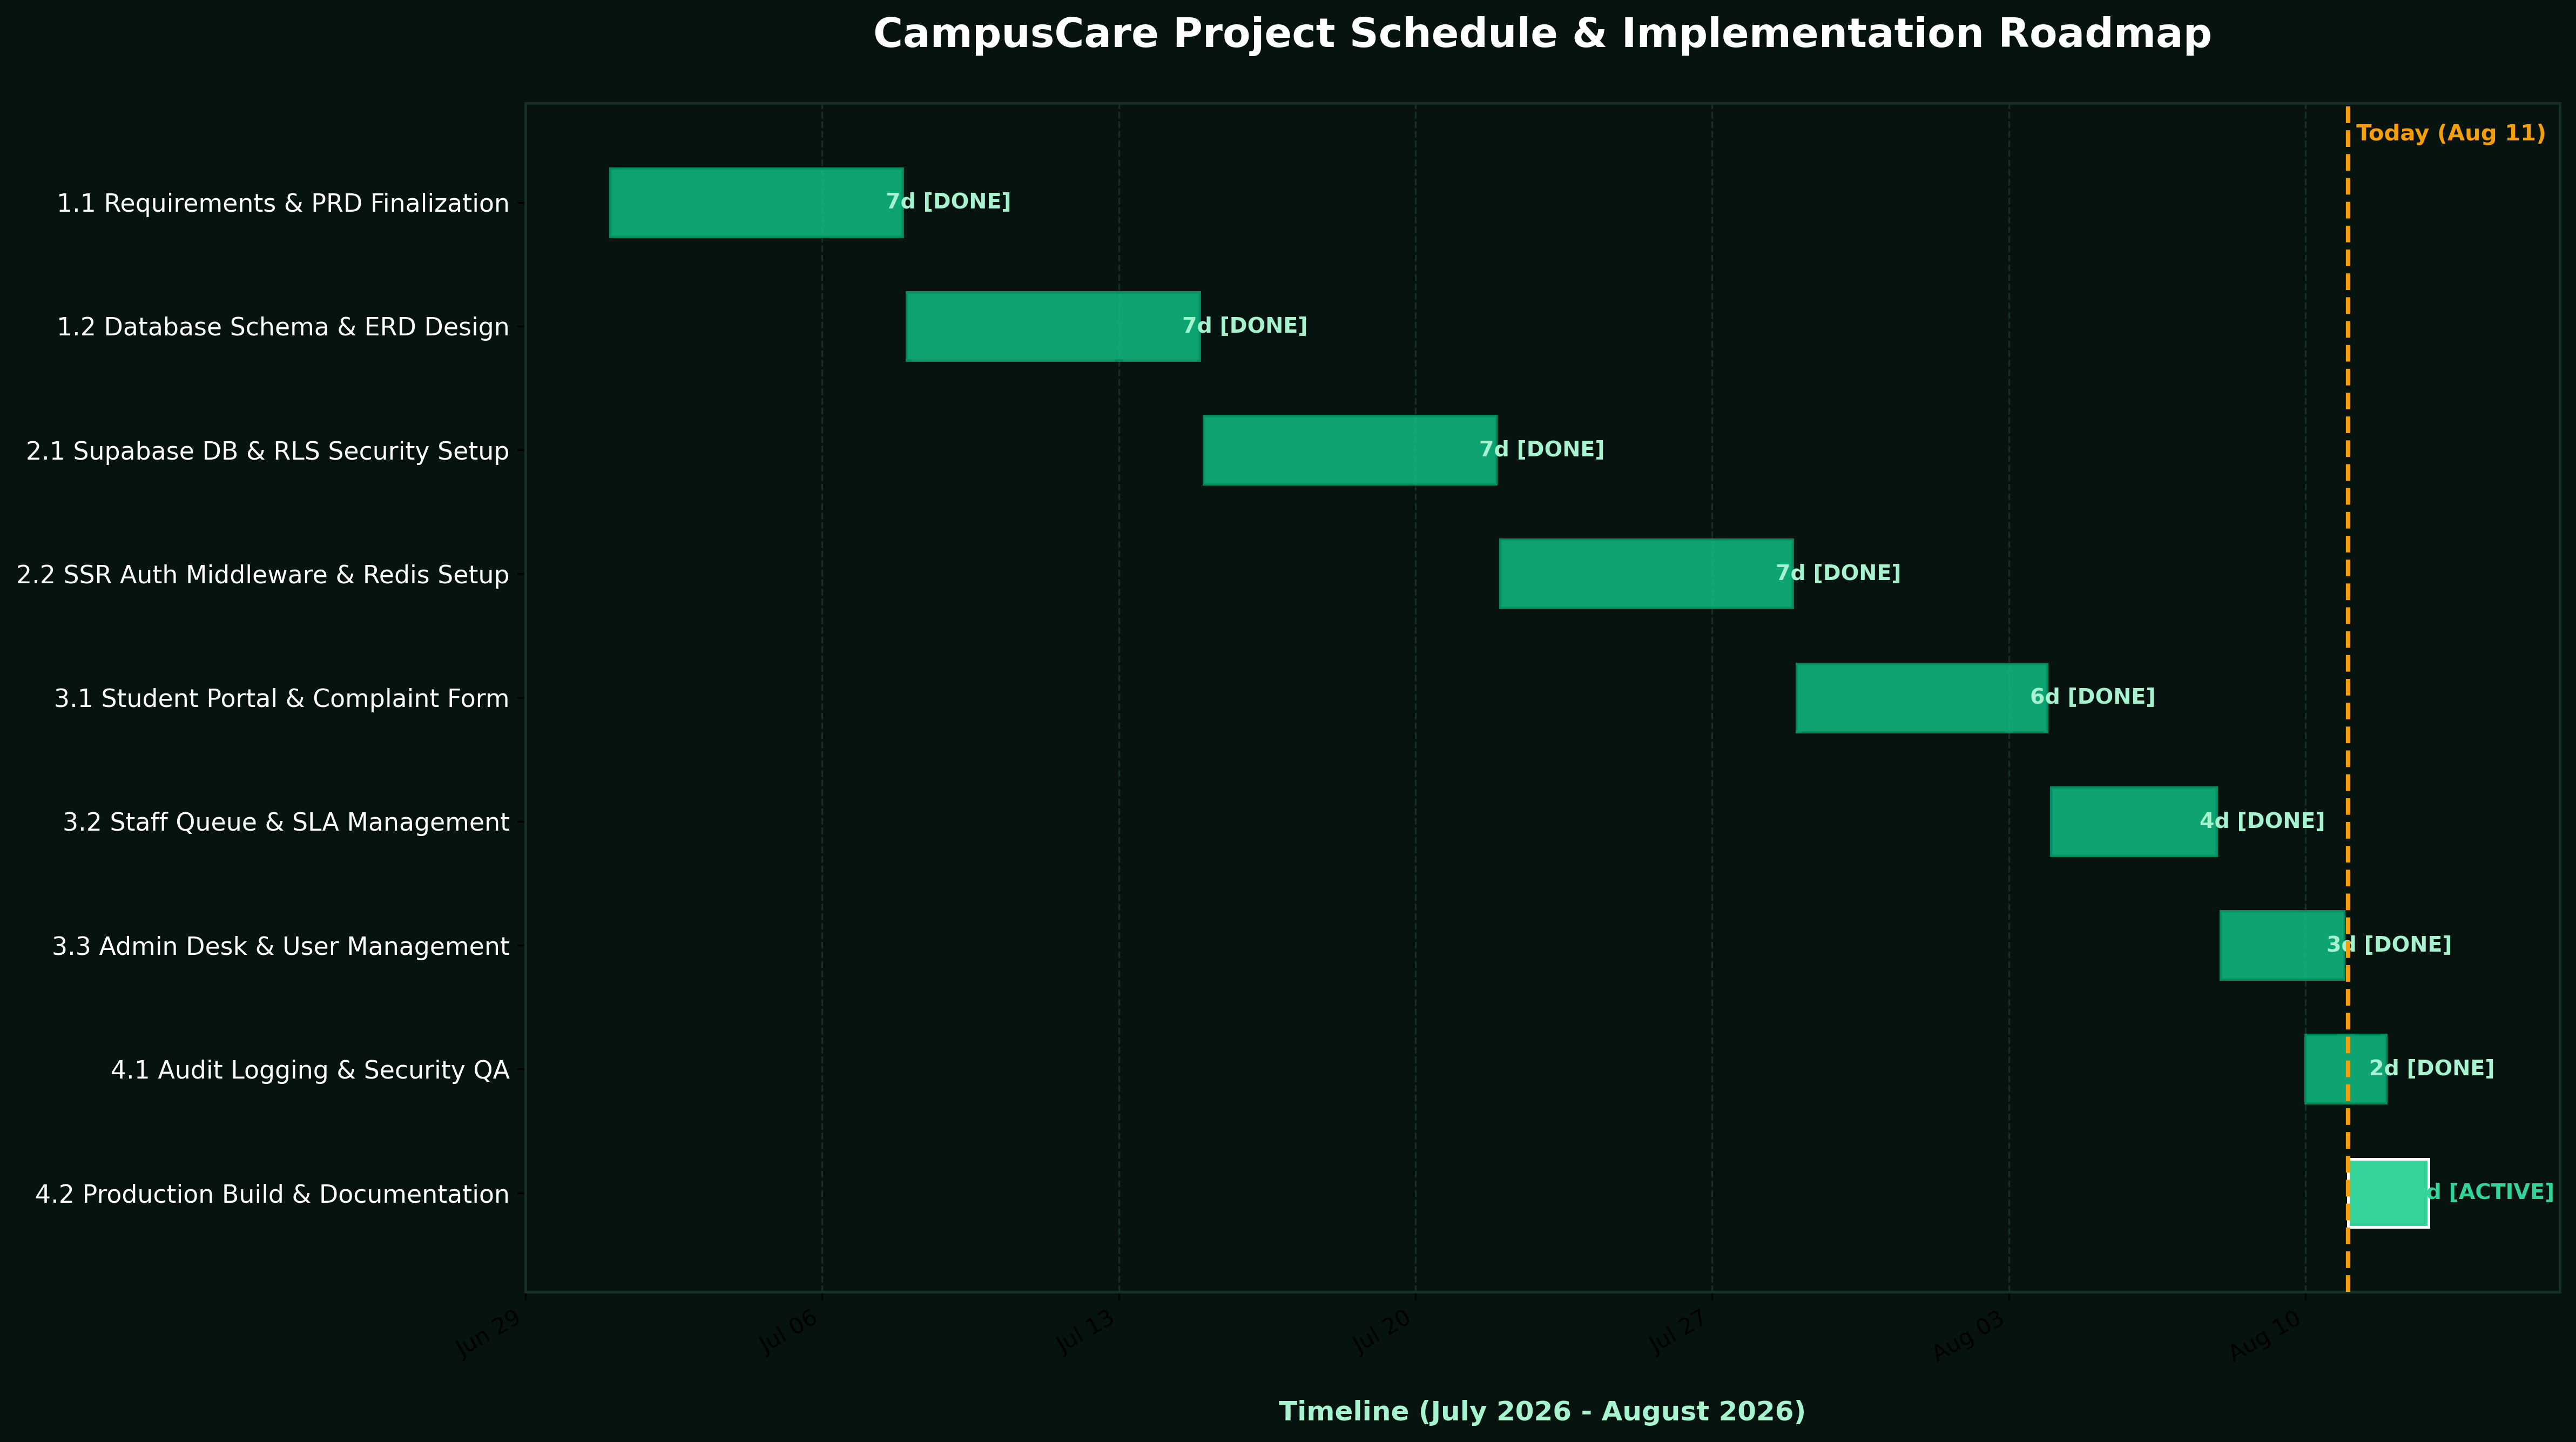
\includegraphics[width=0.95\textwidth]{../diagrams/campuscare_gantt.png}
    \caption{CampusCare Project Implementation Schedule and Gantt Chart.}
    \label{fig:gantt}
\end{figure}

\newpage

% =========================================================
% 6. BUDGET
% =========================================================
\section{Budget and Cost Estimation}

\begin{table}[H]
\centering
\small
\begin{tabularx}{\textwidth}{p{0.24\textwidth} X c r}
\toprule
\textbf{Category} & \textbf{Component / Resource} & \textbf{Quantity} & \textbf{Annual Cost (USD)} \\
\midrule
Development & Internal Engineering Team & 1 Team & \$0.00 \\
Application Hosting & Vercel Hosting (Pro Tier) & 12 Months & \$240.00 \\
Database and Auth & Supabase Managed PostgreSQL (Pro Tier) & 12 Months & \$300.00 \\
Rate Limiting & Upstash Redis Cloud & 12 Months & \$120.00 \\
Domain and Network & Campus Subdomain (\texttt{campuscare.\allowbreak university.edu}) & 1 Domain & \$0.00 \\
SSL Certificate & Vercel / Let's Encrypt Automated SSL & 1 Certificate & \$0.00 \\
Buffer / Storage & Bandwidth and Storage Contingency Buffer & 1 & \$100.00 \\
\midrule
\multicolumn{3}{l}{\textbf{Total Annual Cost}} & \textbf{\$760.00} \\
\bottomrule
\end{tabularx}
\caption{Annualized Cloud Infrastructure and Operational Budget Breakdown.}
\end{table}

\end{document}
